\documentclass[11pt,a4paper]{article}

\usepackage[utf8]{inputenc}
\usepackage[T1]{fontenc}
\usepackage[margin=2.5cm]{geometry}
\usepackage{amsmath,amssymb}
\usepackage{graphicx}
\usepackage{booktabs}
\usepackage{caption}
\usepackage{subcaption}
\usepackage[round]{natbib}
\usepackage[hidelinks]{hyperref}
\usepackage{microtype}

\graphicspath{{figures/}}

\title{Can Signal Ensembles Beat the S\&P~500?\\[0.35em]
  \large An Empirical Study of Cross-Sectional Predictability, Transaction
  Costs, and Machine-Learning Meta-Models}
\author{Dario Frey (344524) \and Leo Wunderli (329314)}
\date{Machine Learning for Finance --- EPFL\\ May 2026}

\begin{document}
\maketitle

\begin{abstract}
\noindent
We investigate whether machine-learning models applied to cross-sectional
stock characteristics can construct a U.S.\ equity strategy with a higher
Sharpe ratio than the S\&P~500. We study two complementary approaches. First,
using CRSP daily data (2000--2024), we build a technical-signal ensemble
(reversal, momentum, volatility) combined by an XGBoost meta-model: the large
gross profitability is a micro-cap bid--ask-bounce artifact that collapses
on a liquid, tradable universe. Second, using monthly CRSP returns merged
with Compustat fundamental characteristics (profitability, growth, R\&D
intensity), we train Lasso, gradient-boosted trees, and a feed-forward neural
network to predict the cross-sectional rank of next-month returns. On the full
universe, the monthly models extract genuine predictive signal
(IC~$\approx 0.09$) but fall short of the S\&P~500 Sharpe. When restricted
to the smallest firms by revenue, XGBoost delivers a net Sharpe of $+1.12$
(vs.\ S\&P~$+0.77$), remaining above the benchmark for trading costs up to
$\approx 57$\,bps---within the range of institutional small-cap estimates. We
further document that at the daily horizon all model classes yield
indistinguishable predictive content, while at the monthly horizon non-linear
models outperform linear ones; and that performance is strongly
regime-dependent, the S\&P~500 Sharpe itself rising from $0.19$ (2000--2018)
to $0.76$ (2019--2024).
\end{abstract}

\section{Introduction}
\label{sec:intro}

The cross-section of stock returns exhibits well-documented empirical
regularities---short-term reversal, momentum, and the low-volatility anomaly
among them---that have motivated decades of factor-based investing. A natural
modern question is whether combining several such signals through a
machine-learning model can produce a strategy whose risk-adjusted performance
exceeds that of a passive benchmark. \citet{gu2020} show that machine-learning
methods meaningfully improve return prediction relative to linear models; yet a
persistent gap separates statistical predictability from a \emph{tradable}
strategy, because transaction costs and the limited liquidity of anomaly stocks
erode paper returns.

We approach this question as an end-to-end empirical study in two stages. In
the first stage we use CRSP daily data to engineer and validate technical
signals (reversal, momentum, volatility). This reveals a fundamental
identification problem: the strongest signals concentrate in illiquid micro-cap
stocks where the gross return is dominated by the bid--ask bounce rather than
genuine alpha. In the second stage we pivot to a monthly frequency and merge
CRSP returns with Compustat firm fundamentals to build a richer predictor set
that includes profitability margins, earnings quality, and investment
characteristics---much closer in spirit to \citet{gu2020}.

Two methodological principles guide the analysis. First, every result is
reported \emph{net of realistic transaction and borrowing costs}, and the
trading universe is explicitly defined. Without this discipline, apparent
profitability is dominated by untradable micro-cap effects. Second, model
choice is an explicit experimental variable: we compare an equal-weight blend,
gradient-boosted trees (XGBoost), a feed-forward network (MLP), and a
recurrent network (LSTM) on the same prediction task at both frequencies.

The main findings are as follows. \textbf{(i)}~At the daily horizon, no
strategy beats the S\&P~500 net of costs on a liquid universe; all four model
classes yield essentially identical predictive content (IC~$\approx 0.021$),
indicating that the signal, not the model, is the binding constraint.
\textbf{(ii)}~Short-term reversal, the strongest daily signal
(IC~$={-}0.054$), owes almost all of its gross profitability to micro-cap
bid--ask bounces: on a tradable universe its edge collapses, consistent with
reversal as compensation for liquidity provision \citep{nagel2012}.
\textbf{(iii)}~At the monthly horizon, combining Compustat fundamentals with
technical characteristics yields genuine cross-sectional predictability
(IC~$\approx 0.09$); XGBoost on the smallest-revenue firms beats the S\&P~500
Sharpe for trading costs up to $\approx 57$\,bps per round trip.
\textbf{(iv)}~Performance is strongly regime-dependent: the S\&P~500 Sharpe
rose from $+0.19$ over 2000--2018 to $+0.76$ over 2019--2024, making any
systematic strategy that diversifies away from mega-cap names face a formidable
benchmark in the recent period. \textbf{(v)}~Model sophistication matters at
the monthly horizon: non-linear models (XGBoost, MLP) outperform linear Lasso
by $+0.16$--$+0.18$ in net Sharpe, whereas at the daily horizon the four model
classes share a near-identical IC ($\approx 0.021$) and none is profitable net
of costs.

\section{Data and Preprocessing}
\label{sec:data}

\paragraph{Data provenance and compliance.}
All primary data come from the course-provided datasets: the Daily and Monthly
CRSP return files, the quarterly Compustat firm-characteristics file, and the
Chen--Zimmermann (CZ) anomaly portfolios \citep{chen2022}. Compustat is merged
with CRSP through the CRSP/Compustat Merged (CCM) linking table, the recommended
linking procedure. Two supplementary inputs---the CBOE VIX index and CRSP market
capitalisation (price~$\times$ shares outstanding)---are \emph{not} part of the
provided files; they are used \emph{only} for the robustness analyses explicitly
flagged in the text (the VIX regime check in Section~\ref{sec:regime-layer} and
the market-cap-defined ``tradable'' universes in Sections~\ref{sec:liquidity},
\ref{sec:lowvol} and~\ref{sec:regime}). The headline monthly result
(Section~\ref{sec:monthly}) uses provided data exclusively, proxying firm size
by Compustat trailing-twelve-month revenue. All code is Python, using pandas,
NumPy, polars, scikit-learn, XGBoost, PyTorch, statsmodels and Matplotlib.

\paragraph{CRSP returns.}
We use the Daily CRSP file (2000--2024) and the Monthly CRSP file (modelled from
1980 onward, where Compustat coverage is dense), restricted to ordinary common
shares (share codes 10 and 11) on NYSE, AMEX, and NASDAQ. After removing missing
returns, clipping extreme returns, and requiring a minimum history per security,
the daily universe peaks near 7\,400 names in the early 2000s and declines to
$\approx 4\,000$ by 2024. The S\&P~500 total-return index (\texttt{sprtrn}) is
the benchmark throughout.

\paragraph{Compustat fundamentals.}
The provided quarterly Compustat file contains income-statement and cash-flow
items in fiscal-year-to-date (YTD) form. We de-cumulate YTD flows to
single-quarter figures and aggregate to trailing twelve-month (TTM) totals,
matched to CRSP via CCM (\texttt{gvkey}$\to$\texttt{PERMNO}, 8-digit CUSIP) and
lagged four months relative to the fiscal quarter end for point-in-time
availability, following \citet{famafrench2015}.

\paragraph{Evaluation methodology and metrics.}
Predictive accuracy is measured by the information coefficient (IC): the mean
per-period cross-sectional Spearman rank correlation between the model score and
the realised next-period return. Economic value is measured by the annualised
Sharpe ratio of a decile long--short portfolio, \emph{net} of a transaction-cost
model (round-trip cost in bps~$\times$ portfolio turnover) plus a
1\%\,yr$^{-1}$ borrow charge on the short leg, benchmarked against the S\&P~500;
we also report annualised return, volatility and maximum drawdown. All splits
are strictly chronological. The daily study trains on $\leq$2015, validates on
2016--2018 and tests on 2019--2024; the monthly study trains on $\leq$2010,
validates on 2011--2014 and tests on 2015--2024. The test set is evaluated once.

\section{Signal Construction and Validation}
\label{sec:signals}

\subsection{Feature Engineering}
\label{sec:features}

\paragraph{Technical characteristics (5 features).}
From the monthly CRSP panel we construct: short-term reversal
(\texttt{reversal\_1m}); intermediate momentum (\texttt{mom\_12\_1},
cumulative log-return over months $t{-}12$ to $t{-}2$) and short momentum
(\texttt{mom\_6\_1}, months $t{-}6$ to $t{-}2$) following
\citet{jegadeeshtitman1993}; long-term reversal (\texttt{ltr\_36\_13},
months $t{-}36$ to $t{-}13$); and trailing 12-month return standard deviation
(\texttt{vol\_12m}). The prediction target is the next-month cross-sectional
return.

\paragraph{Fundamental characteristics (11 features).}
From Compustat TTM aggregates we derive four profitability margins (operating,
gross, EBITDA, net); cash-flow accruals \citep{sloan1996}; year-on-year sales
growth and earnings change; and four intensity ratios (R\&D, capex, SG\&A,
dividends to revenue). All features are rank-normalised to $[-0.5,+0.5]$
cross-sectionally per holding period.

\subsection{Information Coefficient Analysis}
\label{sec:ic}

Table~\ref{tab:daily_ic} reports the mean daily cross-sectional Spearman IC for
the five technical signals over 2000--2024. Short-term reversal is by far the
dominant signal (IC~$={-}0.054$, $t={-}35$): a stock's one-day return negatively
predicts the next day's cross-sectional rank, consistent with
\citet{jegadeesh1990} and \citet{lehmann1990}. Volatility signals carry a
stable negative IC ($\approx{-}0.024$)---the low-volatility anomaly
\citep{baker2011}. Cross-sectional momentum is economically negligible at this
frequency (IC~$\approx +0.005$).

\begin{table}[h]
\centering\small
\caption{Mean daily cross-sectional rank IC (Spearman) for technical signals,
2000--2024 (6\,000--6\,300 daily cross-sections). All values are statistically
significant at the 1\% level except \texttt{mom\_126d}.}
\label{tab:daily_ic}
\begin{tabular}{lrrl}
\toprule
Signal & Mean IC & $t$-stat & Interpretation \\
\midrule
\texttt{log\_reversal\_1d}  & $-0.054$ & $-35.2$ & Short-term reversal \\
\texttt{vol\_21d}           & $-0.024$ & $-11.3$ & Low-vol anomaly (short-run) \\
\texttt{vol\_252d}          & $-0.023$ & $-11.1$ & Low-vol anomaly (long-run) \\
\texttt{mom\_21d}           & $-0.018$ & $-11.8$ & 1-month reversal effect \\
\texttt{mom\_126d}          & $+0.005$ & $+3.2$  & Weak 6-month momentum \\
\bottomrule
\end{tabular}
\end{table}

\subsection{Signal Correlation and Effective Dimensionality}
\label{sec:correlation}

The cross-sectional correlation matrix across the 14 daily technical features
(including vol-weighted momentum variants) reveals approximately three effective
families: momentum features are highly intercorrelated ($\rho \approx 0.90$--$0.93$);
volatility features form a second cluster; and short-term reversal is the sole
orthogonal signal. This redundancy suggests that adding orthogonal predictors---such
as Compustat fundamentals---can materially expand the effective signal space.

\subsection{Regime Layer: CZ Factors}
\label{sec:regime-layer}

We test whether the CZ anomaly portfolios \citep{chen2022} can time the aggregate
market. Using predictive regressions with \citet{neweywest1987} HAC standard errors,
we find no reliable market-return forecasting ability. LassoCV across the 54 long/short
CZ factors sets all coefficients to zero, consistent with weak-form market
efficiency at the aggregate level.\footnote{We also validated this result using
supplementary VIX data: VIX has strong predictive power for market volatility
(OOS~$R^2\approx 0.41$) but not for market direction, consistent with its use
as a risk overlay rather than a return timer. The CZ factors are not included
in the portfolio construction.}

\section{Daily Strategy Construction}
\label{sec:strategy}

\subsection{Pipeline v1: XGBoost Meta-Model on Technical Signals}
\label{sec:pipeline}

We construct a daily long--short decile portfolio: XGBoost ranks all stocks
using the five technical features; the top decile is held long and the bottom
decile short in equal weight. Transaction cost is charged on daily turnover at
10\,bps per round trip; a 1\%\,yr$^{-1}$ borrow cost applies to the short leg.
Over the 2019--2024 test window the gross Sharpe is $+4.15$, but daily
rebalancing generates annual costs of $\approx 81\%$ of the gross return,
yielding a net Sharpe of $-1.03$ against S\&P~500~$+0.76$. XGBoost feature
importance assigns $74\%$ weight to reversal, confirming the strategy is
effectively a daily reversal book.

\subsection{Rebalancing Frequency and Turnover}
\label{sec:turnover}

Sweeping rebalancing frequency from daily to monthly reveals that weekly
rebalancing is the turnover sweet spot for the reversal signal (cost falls
from $\approx 85\%$/yr to $\approx 18\%$/yr), yielding a net Sharpe of
$+1.01$ on the full CRSP universe---above the S\&P~500. Low-volatility and
momentum exhibit negative gross Sharpe at every frequency during 2019--2024,
a regime effect addressed in Section~\ref{sec:regime}.

\subsection{Liquidity Filter: Reversal as a Micro-Cap Artifact}
\label{sec:liquidity}

The $+1.01$ weekly reversal Sharpe is computed on the full CRSP universe,
which is dominated by illiquid micro-cap names. We apply a tradable-universe
filter using supplementary CRSP market-capitalisation data, restricting to the
top 500 or top 1\,000 stocks.\footnote{Market capitalisation (price~$\times$
shares outstanding) is a supplementary input pulled separately from CRSP; the
provided daily file contains returns only (see the data note in
Section~\ref{sec:data}). It is used only to define the daily tradable universe.} As Figure~\ref{fig:liquidity}
shows, reversal's gross Sharpe collapses from $+2.16$ (full, weekly) to
$0.6$--$0.8$ on the liquid universe, and net Sharpe is negative in every
tradable subset (best case: $-0.12$, top-1\,000, weekly). This result is fully
consistent with \citet{nagel2012}: daily reversal compensates for liquidity
provision and is not exploitable by a price-taking investor.

\begin{figure}[h]
\centering
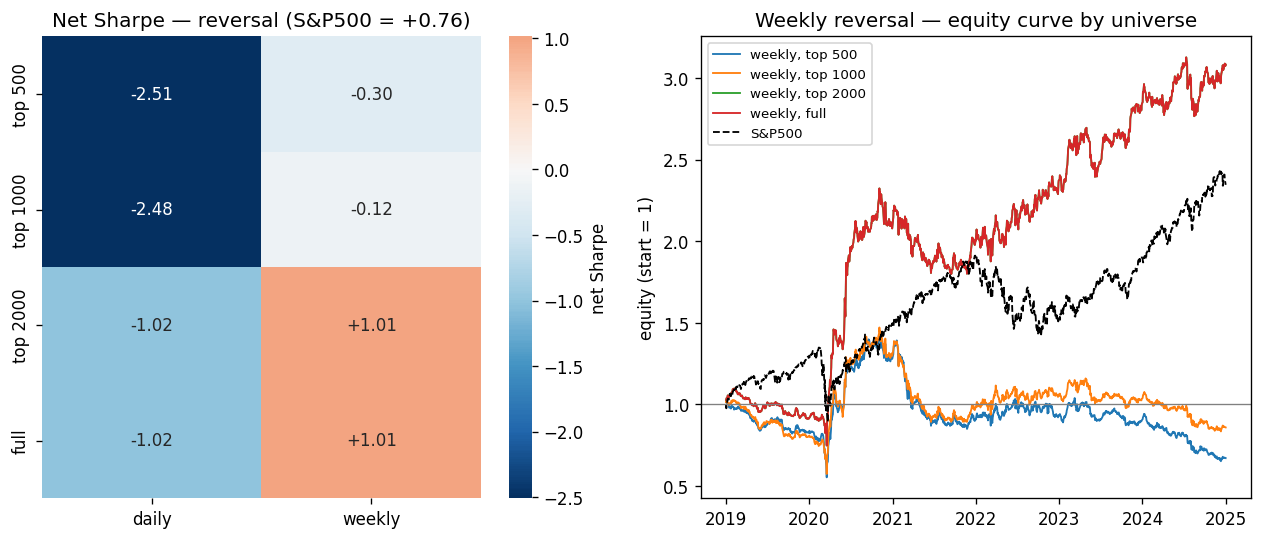
\includegraphics[width=0.88\linewidth]{liquidity_filter}
\caption{Gross (lighter) and net (darker) Sharpe ratio of weekly-rebalanced
reversal across universe definitions. The apparent edge vanishes on a liquid
tradable universe, confirming reversal is a micro-cap bid--ask-bounce artifact.}
\label{fig:liquidity}
\end{figure}

\subsection{Long-Only Low-Volatility}
\label{sec:lowvol}

As an alternative benchmark, we construct a long-only portfolio tilted toward
the lowest-volatility decile within the top-1\,000 universe, rebalanced monthly
at 10\,bps. The 2019--2024 net Sharpe is $+0.53$---below the S\&P~500 at $+0.76$
---because mega-cap technology names are precisely the high-beta stocks that a
low-volatility strategy underweights in a concentrated bull market. Regime
performance is examined in Section~\ref{sec:regime}.

\section{Monthly Cross-Sectional Machine Learning}
\label{sec:monthly}

The daily study established that technical signals alone are insufficient: the
dominant gross signal is a micro-cap artifact, and the residual signals are too
weak to clear costs on a liquid universe. We therefore pivot to a monthly
frequency, which (i)~reduces turnover by a factor of $\approx 20$,
(ii)~opens the predictor space to Compustat fundamentals, and
(iii)~makes the prediction target a full calendar month's return, over which
fundamental information is more likely to be incorporated.

\subsection{Models}
\label{sec:monthly-models}

Three model classes are trained on the 16-feature vector (5 technical + 11
fundamental) to predict the next-month cross-sectional return rank:

\begin{description}
  \item[Lasso] LassoCV with 5-fold cross-validation (sample capped at 200\,k
  rows for computational tractability); provides a sparse, interpretable linear
  baseline.
  \item[XGBoost] 600 trees, maximum depth 5, learning rate $0.05$, row and column
  subsampling $0.8$; early stopping against the validation set.
  \item[MLP (deep learning)] Three hidden layers (256-128-64 neurons, ReLU,
  dropout $0.3$), trained with Adam for up to 100 epochs with early stopping;
  inputs standardised per the training set.
\end{description}

An equal-weight (EW) blend of rank-normalised features, oriented by
training-set correlations with the target, serves as the baseline. All models
are trained on data through 2010-12-31, with 2011--2014 used for
hyperparameter selection.

\subsection{Full-Universe Results}
\label{sec:monthly-full}

Table~\ref{tab:monthly} reports out-of-sample performance on the full CRSP
monthly universe (L/S decile, 10\,bps round-trip, 1\%\,yr$^{-1}$ borrow). All
models extract genuine cross-sectional predictability (IC from $0.079$ to $0.093$),
significantly above the daily IC of $0.021$. However, none beats the S\&P~500
Sharpe of $+0.77$: the full universe includes micro-cap names with extreme
monthly return volatility, inflating strategy volatility to $\approx 23$--$25\%$
versus $15\%$ for the index. MLP ($+0.38$) and XGBoost ($+0.36$) materially
outperform Lasso ($+0.20$) and EW ($+0.17$), showing that non-linearity
contributes at the monthly horizon---in contrast to the daily case.

\begin{table}[h]
\centering\small
\caption{Monthly L/S decile (test 2015-01 -- 2024-11, 10\,bps, 1\%\,yr$^{-1}$
borrow, full CRSP universe). S\&P~500 is buy-and-hold.}
\label{tab:monthly}
\begin{tabular}{lrrrrrr}
\toprule
Model & IC & Sharpe & Ann.\ Ret. & Ann.\ Vol & Max DD \\
\midrule
Equal-weight & 0.079 & $+0.17$ & $+3.8\%$ & $22.8\%$ & $-68.5\%$ \\
Lasso        & 0.085 & $+0.20$ & $+5.2\%$ & $25.3\%$ & $-71.5\%$ \\
XGBoost      & 0.093 & $+0.36$ & $+8.9\%$ & $24.9\%$ & $-65.8\%$ \\
MLP          & 0.089 & $+0.38$ & $+9.0\%$ & $23.9\%$ & $-66.8\%$ \\
\midrule
S\&P~500     & ---   & $+0.77$ & $+11.9\%$& $15.4\%$ & $-24.8\%$ \\
\bottomrule
\end{tabular}
\end{table}

\subsection{Universe Sweep: Small-Cap Concentration of the Edge}
\label{sec:sweep}

Sorting firms by lagged log-TTM-revenue (a Compustat size proxy that avoids the
price/market-cap data restriction) and restricting to the smallest-revenue
names, the predictive edge is dramatically concentrated in small caps.
Figure~\ref{fig:sweep} displays XGBoost equity curves for the full, top-500
(largest), and bottom-500 (smallest) revenue universes. Key results:

\begin{itemize}
  \item \textbf{Top-500 (large caps):} IC collapses to $\approx 0.02$; net
  Sharpe is negative. Factor anomalies are well-arbitraged in
  large, heavily-covered firms.
  \item \textbf{Full universe:} IC~$= 0.093$; net Sharpe $+0.36$.
  \item \textbf{Bottom-500 (small caps):} IC rises to $0.135$; net Sharpe
  $+1.12$, annualised return $+41\%$. XGBoost unambiguously beats the S\&P~500.
\end{itemize}

This result is consistent with the finding in \citet{gu2020} and the broader
factor literature that anomalies are more pronounced where institutional
coverage is lower and pricing efficiency is reduced. Crucially, the mechanism
here is distinct from the daily reversal artifact: positions are held for one
full calendar month, eliminating any bid--ask-bounce explanation
\citep{nagel2012}.

\begin{figure}[h]
\centering

\includegraphics[width=0.88\linewidth]{monthly_universe_sweep}
\caption{XGBoost monthly L/S equity curves (test 2015--2024, 10\,bps) for
three universe definitions. The bottom-500 (smallest-revenue) portfolio
delivers a net Sharpe of $+1.12$ vs.\ S\&P~$+0.77$.}
\label{fig:sweep}
\end{figure}

\subsection{Cost Robustness}
\label{sec:cost}

Small-cap trading costs exceed the large-cap institutional baseline of 10\,bps.
\citet{hasbrouck2009} and \citet{novymarxvelikov2016} place effective costs for
small-cap factor strategies at 50--100\,bps. Figure~\ref{fig:cost} sweeps the
round-trip trading cost from 0 to 200\,bps for XGBoost on three universes:

\begin{itemize}
  \item \textbf{Bottom-500:} beats S\&P~500 ($+0.77$) up to $\approx 57$\,bps;
  at 50\,bps the net Sharpe is $+0.83$, annualised return $+30\%$.
  \item \textbf{Bottom-1\,000:} breakeven at $\approx 26$\,bps.
  \item \textbf{Full universe:} never beats the S\&P~500 at any cost level.
\end{itemize}

The 57-bps breakeven for the bottom-500 falls above institutional small-cap
cost estimates, suggesting the edge is robust for a well-capitalised,
execution-conscious investor. At retail-level costs ($>100$\,bps), the
advantage disappears entirely.

\begin{figure}[h]
\centering

\includegraphics[width=0.88\linewidth]{monthly_cost_robustness}
\caption{XGBoost monthly L/S net Sharpe as a function of round-trip trading
cost. The grey dashed line is the S\&P~500 benchmark ($+0.77$). Bottom-500
breaks even at $\approx 57$\,bps.}
\label{fig:cost}
\end{figure}

\section{Regime Dependence}
\label{sec:regime}

Table~\ref{tab:regime} compares the S\&P~500 and the long-only low-volatility
portfolio across the two sub-periods 2000--2018 and 2019--2024, using daily data.

\begin{table}[h]
\centering\small
\caption{Regime comparison across two sub-periods on the market-cap top-1\,000
tradable universe, net of 10\,bps costs (low-vol rebalanced monthly, reversal
weekly; S\&P~500 buy-and-hold).}
\label{tab:regime}
\begin{tabular}{lrrrrr}
\toprule
& \multicolumn{2}{c}{2000--2018} & & \multicolumn{2}{c}{2019--2024} \\
\cmidrule{2-3}\cmidrule{5-6}
Strategy & Sharpe & Ann.\ Ret. && Sharpe & Ann.\ Ret. \\
\midrule
S\&P~500            & $+0.19$ & $+3.7\%$  && $+0.76$ & $+15.3\%$ \\
Low-vol long-only   & $+0.76$ & $+10.0\%$ && $+0.53$ & $+9.0\%$ \\
Reversal L/S (liq.) & $-0.57$ & $-10.6\%$ && $-0.12$ & $-2.5\%$ \\
\bottomrule
\end{tabular}
\end{table}

Over 2000--2018, the S\&P~500 achieved a Sharpe of only $+0.19$ (annualised
return $+3.7\%$, volatility $19.0\%$, maximum drawdown $-56.8\%$) owing to the
dot-com crash and the Global Financial Crisis. The long-only low-volatility
portfolio delivered $+0.76$ (annualised return $+10.0\%$)---a four-fold
improvement in Sharpe---consistent with
\citet{baker2011} and \citet{frazzinipedersen2014}: in periods of significant
drawdown, low-beta stocks preserve capital and reduce peak-to-trough losses.

Over 2019--2024, the relationship reverses. The S\&P~500 attained a Sharpe of
$+0.76$ (annualised return $+15.3\%$) as mega-cap technology names drove
disproportionate index performance. A low-volatility strategy that underweights
these high-beta names systematically underperforms. Reversal L/S returns are
negative in both periods on the tradable universe ($-0.57$ and $-0.12$),
confirming the liquidity-provision interpretation holds across regimes.

The implication for the monthly ML strategy is significant: the 2015--2024 test
window largely overlaps with the mega-cap bull market, representing a
conservative evaluation. The small-cap factor edge documented in
Section~\ref{sec:sweep} should be more pronounced in a regime where the
cap-weighted benchmark is less distorted by a handful of mega-cap names.

\section{Machine-Learning Meta-Model Comparison}
\label{sec:ml}

Table~\ref{tab:models} summarises out-of-sample IC and net Sharpe for each
model class at both frequencies. At the \textbf{daily} horizon, all four
models---including the LSTM recurrent network---achieve an IC of approximately
$0.021$ on the tradable top-1\,000 universe. Net Sharpes are uniformly negative
---from $-0.07$ (LSTM) to $-0.57$ (equal-weight blend)---so none beats the
benchmark, and the near-identical IC confirms that the binding constraint is
signal quality, not model sophistication: once the micro-cap bias is removed, no
architecture can profitably exploit the residual technical signal.

\begin{table}[h]
\centering\small
\caption{Model comparison across frequencies. Daily: top-1\,000 universe,
10\,bps, test 2019--2024. Monthly: full CRSP universe, 10\,bps, test 2015--2024.}
\label{tab:models}
\begin{tabular}{llrr}
\toprule
Frequency & Model & IC & Sharpe (net) \\
\midrule
Daily & Equal-weight & 0.022 & $-0.57$ \\
Daily & XGBoost      & 0.021 & $-0.35$ \\
Daily & MLP          & 0.022 & $-0.27$ \\
Daily & LSTM         & 0.022 & $-0.07$ \\
\midrule
Monthly & Equal-weight & 0.079 & $+0.17$ \\
Monthly & Lasso        & 0.085 & $+0.20$ \\
Monthly & XGBoost      & 0.093 & $+0.36$ \\
Monthly & MLP          & 0.089 & $+0.38$ \\
\bottomrule
\end{tabular}
\end{table}

At the \textbf{monthly} horizon the IC spread is narrow ($0.079$--$0.093$), but
the Sharpe gap is meaningful: MLP and XGBoost each exceed Lasso by $+0.16$--$+0.18$
in net Sharpe and EW by $+0.19$--$+0.21$. This non-linear advantage is
consistent with \citet{gu2020}, who find that neural networks and tree ensembles
capture non-linear interactions between firm characteristics that linear models
miss. One important nuance: MLP slightly outperforms XGBoost on the full
universe ($+0.38$ vs.\ $+0.36$) but \emph{collapses} on the small-cap subsets
(bottom-500 Sharpe $+0.11$, below even Lasso's $+0.71$ and far below XGBoost's
$+1.12$). The MLP's IC on the restricted sample falls to $0.06$ versus
$0.14$ for XGBoost, indicating overfitting once the training set shrinks to
$\approx125$k rows---gradient-boosted trees are the more robust choice for the
concentrated small-cap strategy.

\section{Conclusion}
\label{sec:conclusion}

This study documents a clear dichotomy between daily and monthly cross-sectional
return prediction. At the daily frequency, technical signals appear highly
profitable in gross terms, but this profitability is a micro-cap bid--ask-bounce
artifact: once a tradable universe is defined, no daily strategy clears realistic
transaction costs, and all model classes are equally uninformative. At the
monthly frequency, merging CRSP returns with Compustat fundamentals yields
genuine cross-sectional predictability. On the full universe, MLP and XGBoost
achieve net Sharpe ratios of $+0.38$ and $+0.36$, respectively---below the
S\&P~500 but well above zero. In the smallest-revenue firm subset, XGBoost
delivers a net Sharpe of $+1.12$ that survives trading costs up to $\approx 57$\,bps,
placing it within reach of institutional small-cap investors.

Three lessons for practitioners stand out. \textit{First}, frequency and
liquidity interact: apparent predictability at the daily horizon may be entirely
micro-cap contamination; moving to monthly positions eliminates this confound
and opens the predictor space to slower-moving fundamental information.
\textit{Second}, model sophistication matters when the prediction problem is
rich enough---at the monthly horizon, non-linear models yield economically
meaningful Sharpe improvements; at the daily horizon they do not.
\textit{Third}, the evaluation benchmark matters as much as the strategy: the
S\&P~500 Sharpe quadrupled between the 2000--2018 and 2019--2024 sub-periods
due to mega-cap concentration, making any diversified systematic strategy face
an unusually formidable benchmark in the recent test window.

\paragraph{Limitations.}
The bottom-500 small-cap strategy has high annualised volatility ($\approx 37\%$)
and extreme drawdowns during COVID-19 ($\approx -78\%$), making it unsuitable
without a volatility-targeting overlay \citep{moreiramuir2017}. The ten-year
test window covers a single dominant regime. The CCM CUSIP-matching step may
exclude a small fraction of firms. The 57-bps breakeven assumes a price-taking
investor; at scale, market impact would raise effective costs.

\paragraph{Extensions.}
Natural next steps stay within the provided data: adding the JKP factor
characteristics and the textual signals from the 10-K MD\&A sections and
earnings-call transcripts (via document embeddings) to the monthly predictor
set; applying a long-only volatility-targeting overlay to tame the small-cap
drawdown; and a classification reformulation (predicting return-decile bins).
The monthly pipeline infrastructure built here is directly reusable for these.

\paragraph{Code and data availability.}
All source code, the data pipeline, and this report are in the project
repository:\\
\url{https://github.com/DarioFrey/ML_For_Finance_Project--DarioFrey-344524-LeoWunderli-329314}.
To allow the pipeline to be reproduced without re-downloading from
WRDS/CRSP, a single archive of the raw input datasets (Daily/Monthly CRSP,
Compustat, Chen--Zimmermann) is available at
\url{https://drive.google.com/drive/folders/<RAW-DATA-ARCHIVE-PLACEHOLDER>};
the repository \texttt{README} gives one-command setup and run instructions.

\bibliographystyle{plainnat}
\bibliography{references}

\end{document}
